\documentclass[a4paper, 14pt]{extarticle}
\usepackage{enumitem}
\usepackage{fefutitle}
\usepackage{xcolor}
\usepackage{amsmath}
\usepackage{graphicx}
\usepackage[justification=centering]{caption}
\usepackage{float}

\begin{document}
	\fefutitle{4}
	\pagebreak	

	\section{Введение}
		Маятник — система, подвешенная в поле тяжести и совершающая механические колебания. Маятники используются в различных приборах, например, в часах и сейсмографах. Они облегчают изучение колебаний, так как наглядно демонстрируют их свойства. Одним из простейших маятников является шарик, подвешенный на нити. Если считать нить нерастяжимой и пренебречь размерами груза по сравнению с длиной нити, а массой нити по сравнению с массой груза, то шарик на нити можно рассматривать как материальную точку, находящуюся на неизменном расстоянии от точки подвеса. Такой маятник называется математичским.
		
		В данной работе будет реализована модель маятника в нескольких вариантах:
		\begin{enumerate}
			\item Без учёта трения
			\item С учётом трения
			\item C учётом трения и вынужденных колебаний
		\end{enumerate}
		
		
		
	\section{Создание математической модели}
		\begin{figure}[H]
			\centering
			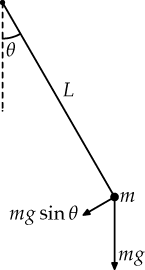
\includegraphics[]{fig1.png}
			\caption[.] {Математический маятник}
		\end{figure}
		
		Момент инерции математического маятника равен:
		\[ M_{\text{ин}} = J\dfrac{d^2\theta}{dt^2} \tag{1} \label{eq:1} \],
		где $\theta$ - угол наклона маятника в текущий момент, $J$ - момент инерции, относительно оси
		
		Момент инерции вычисляется по формуле:
		\[ J = mL^2 \tag{2} \label{eq:2} \], где $m$ - масса маятника, L - длина нити
		
		Если тело не находится в положении равновесия, то на него действует возвращающий момент:
		\[ M_{\text{в}} = FL = -mgL\sin{\theta} \], где $g \approx 9.8$ - ускорение свободного падения
		
		Подставим \eqref{eq:2} в \eqref{eq:1} и приравняем моменты:
		\[ mL^2\dfrac{d^2\theta}{dt^2} = -mgL\sin{\theta} \] 
		
		Сделаем элементарные преобразования, примем $\omega_0 = \dfrac{g}{L}$ и получим нелинейное дифференциальное уравнение второго порядка, описывающее маятник:
		\[ \ddot{\theta} + \omega_0^2 \cdot \sin{\theta} = 0 \]
		
		Для решения понизим порядом и сведем к системе дифференциальных уравнений первого порядка:
		\[\begin{cases}
			\dot{\theta} = \upsilon, \\
			\dot{\upsilon} + \omega_0^2\sin{\theta} = 0
		\end{cases}\]
		
		При малых углах \( \sin{\theta} \approx \theta \) и уравнение превращается в
		\[ \ddot{\theta} + \omega_0^2 \cdot \theta = 0, \]
		с соответсвующей ей системой:
		\[\begin{cases}
			\dot{\theta} = \upsilon, \\
			\dot{\upsilon} + \omega_0^2\theta = 0
		\end{cases}\]
		
		При наличии затуханий уравнение примет вид:
		\[ \ddot{\theta} + k \dot{\theta} + \omega_0^2\sin{\theta} = 0, \]
		где k - коэффициент затухания
		
		с соответсвующей ей системой:
		\[\begin{cases}
			\dot{\theta} = \upsilon, \\
			\dot{\upsilon} + k\upsilon +\omega_0^2\sin{\theta} = 0
		\end{cases}\]
		
		Добавим внешнюю периодическую силу, действующую на маятник, и колебания станут вынужденными:
		\[ \ddot{\theta} + k \dot{\theta} + \omega_0^2\sin{\theta} = a \cdot \sin{(\omega t)}, \]
		
		с соответсвующей ей системой:
		\[\begin{cases}
			\dot{\theta} = \upsilon, \\
			\dot{\upsilon} + k\upsilon +\omega_0^2\sin{\theta} = a\sin{(\omega t)}
		\end{cases}\]
	
	\pagebreak
	\section{Реализация модели}
		Модель была реализована в MathCad.
		\subsection{Сравнение линейных и нелинейных незатухающих колебаний}		
		\begin{figure}[H]
			\centering
			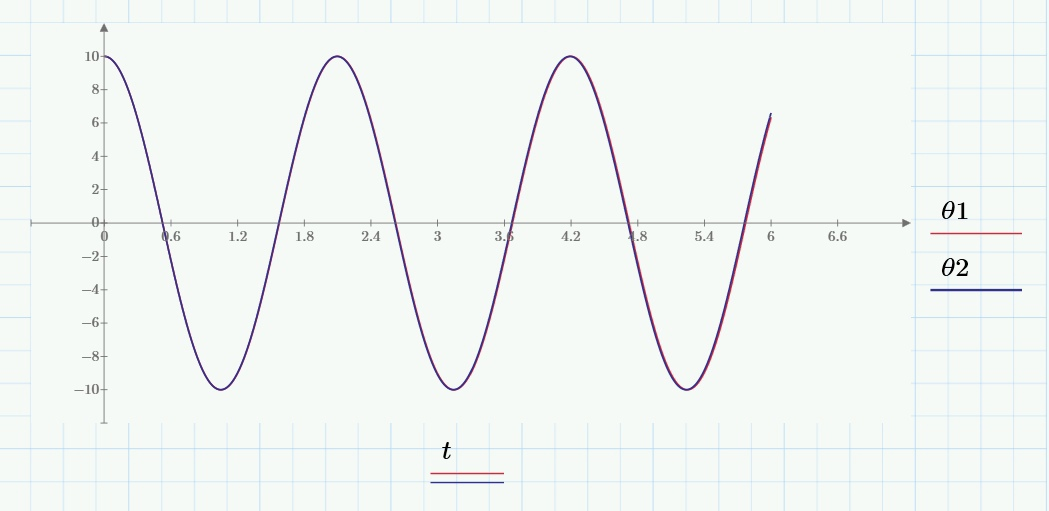
\includegraphics[width = \linewidth]{2.jpg}
			\caption[.] {График сравнения линейных и нелинейных колебаний при $\theta = 10^{\circ}$}
		\end{figure}
		\begin{figure}[H]
			\centering
			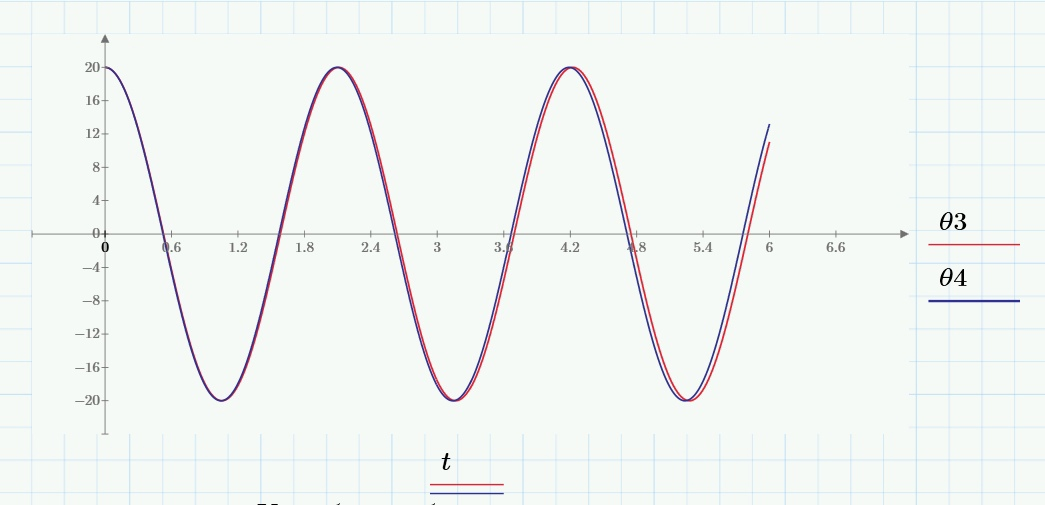
\includegraphics[width = \linewidth]{4.jpg}
			\caption[.] {График сравнения линейных и нелинейных колебаний при $\theta = 20^{\circ}$}
		\end{figure}
		\begin{figure}[H]
			\centering
			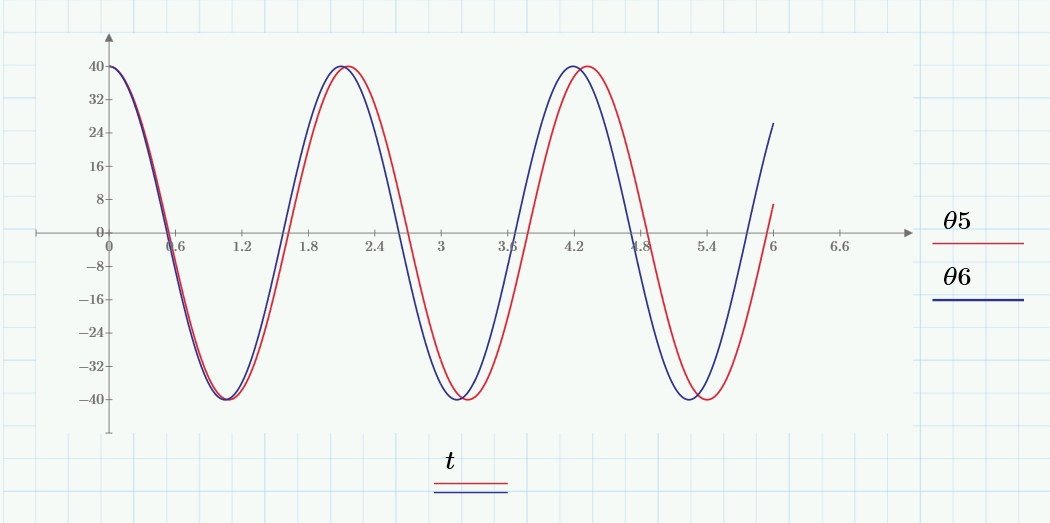
\includegraphics[width = \linewidth]{6.jpg}
			\caption[.] {График сравнения линейных и нелинейных колебаний при $\theta = 40^{\circ}$}
		\end{figure}
		\begin{figure}[H]
			\centering
			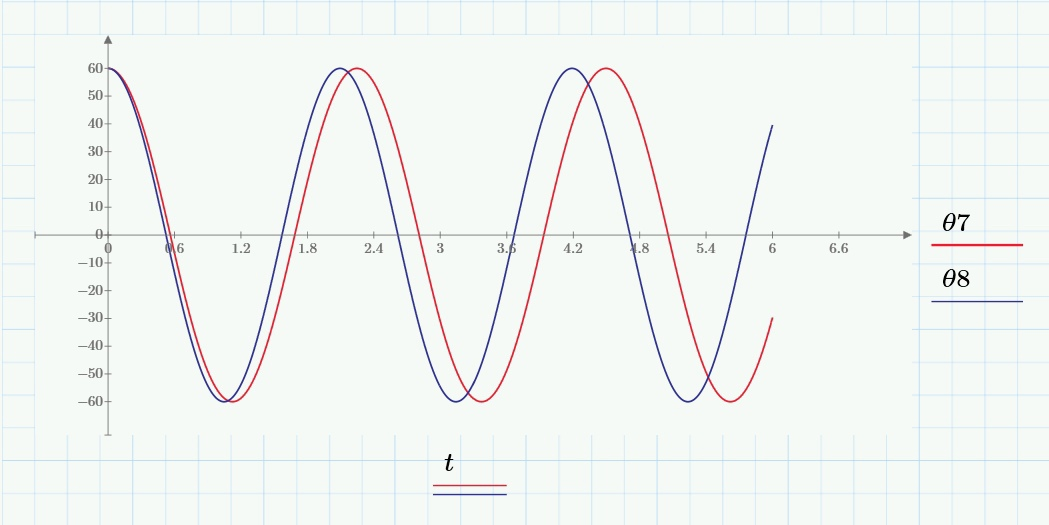
\includegraphics[width = \linewidth]{8.jpg}
			\caption[.] {График сравнения линейных и нелинейных колебаний при $\theta = 60^{\circ}$}
		\end{figure}	
		\begin{figure}[H]
			\centering
			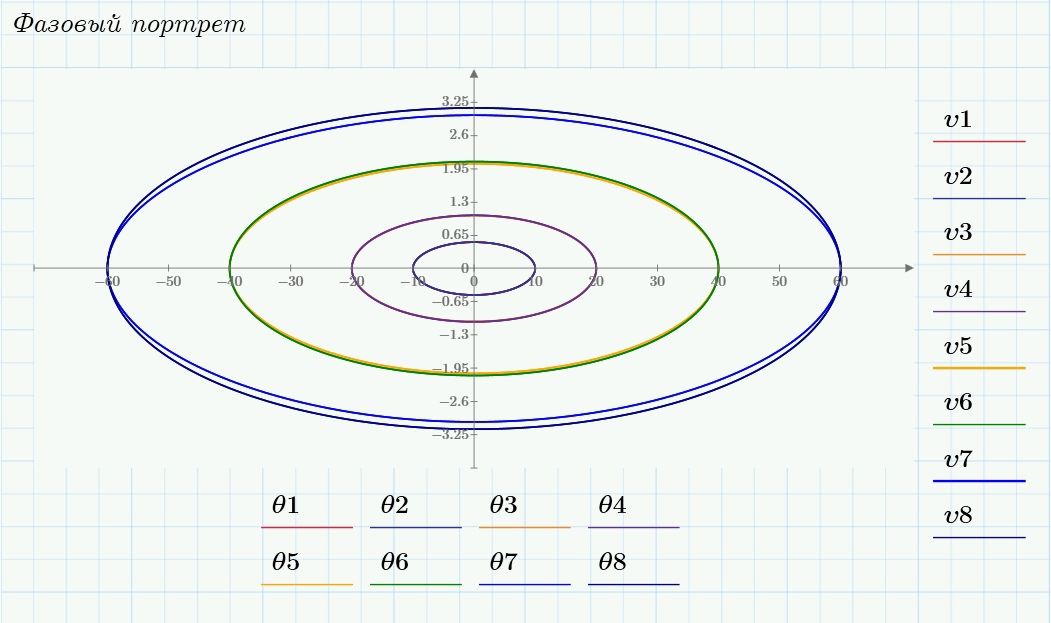
\includegraphics[width = \linewidth]{9.jpg}
			\caption[.] {Фазовый портрет колебаний при разных углах}
		\end{figure}
	\subsection{Затухающие колебания}	
		\begin{figure}[H]
			\centering
			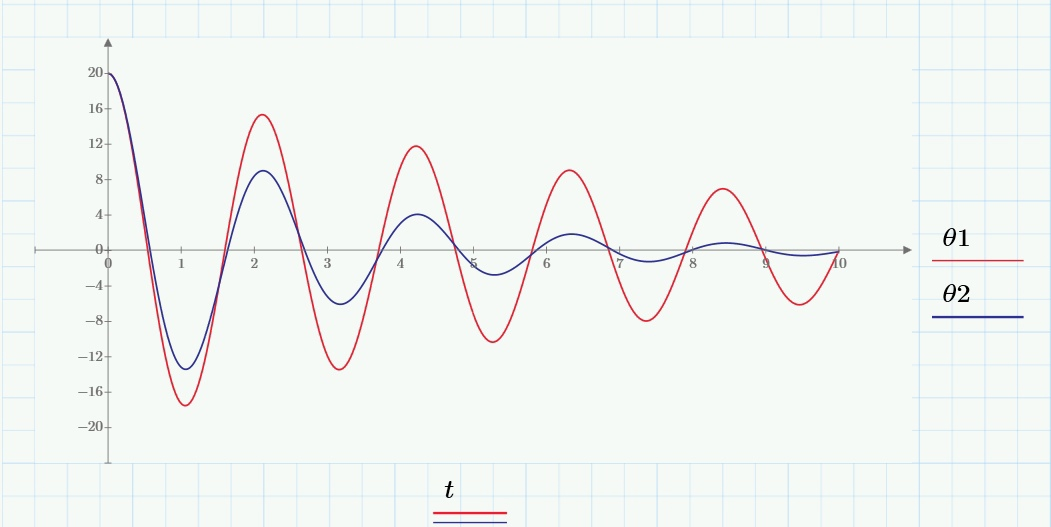
\includegraphics[width = \linewidth]{11.jpg}
			\caption[.] {График колебаний при $\theta = 20^{\circ}$ $k = 0.25$ и $k=0.75$}
		\end{figure}
		\begin{figure}[H]
			\centering
			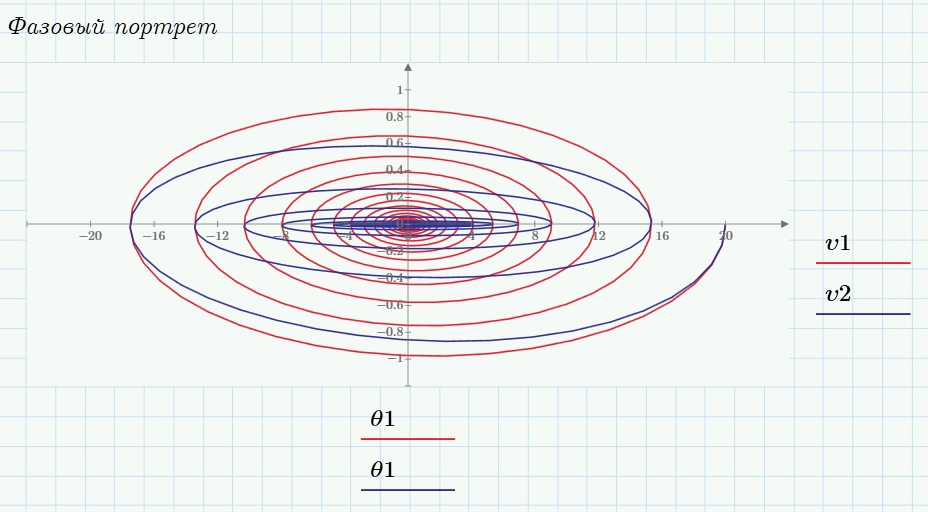
\includegraphics[width = \linewidth]{12.jpg}
			\caption[.] {Фазовый портрет при $\theta = 20^{\circ}$ $k = 0.25$ и $k=0.75$}
		\end{figure}
		\begin{figure}[H]
			\centering
			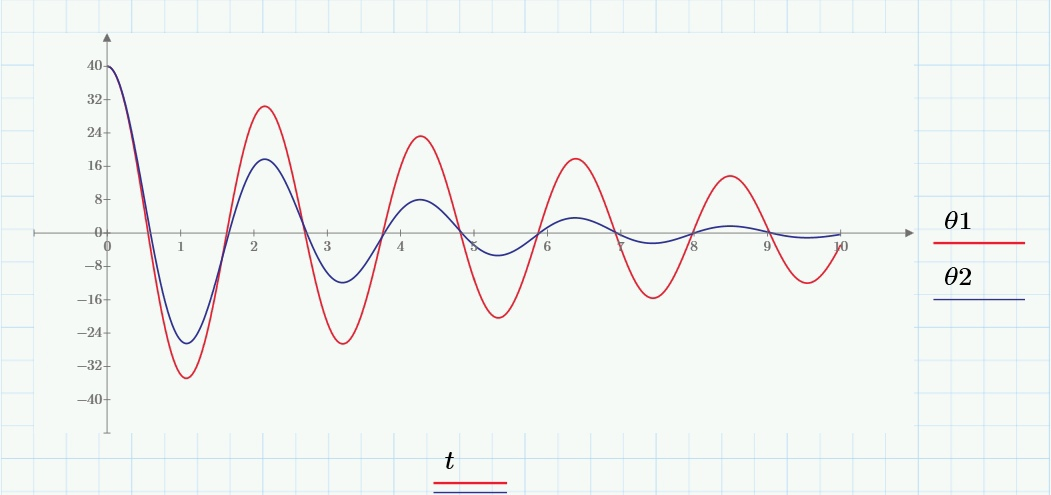
\includegraphics[width = \linewidth]{14.jpg}
			\caption[.] {График колебаний при $\theta = 40^{\circ}$ $k = 0.25$ и $k=0.75$}
		\end{figure}
		\begin{figure}[H]
			\centering
			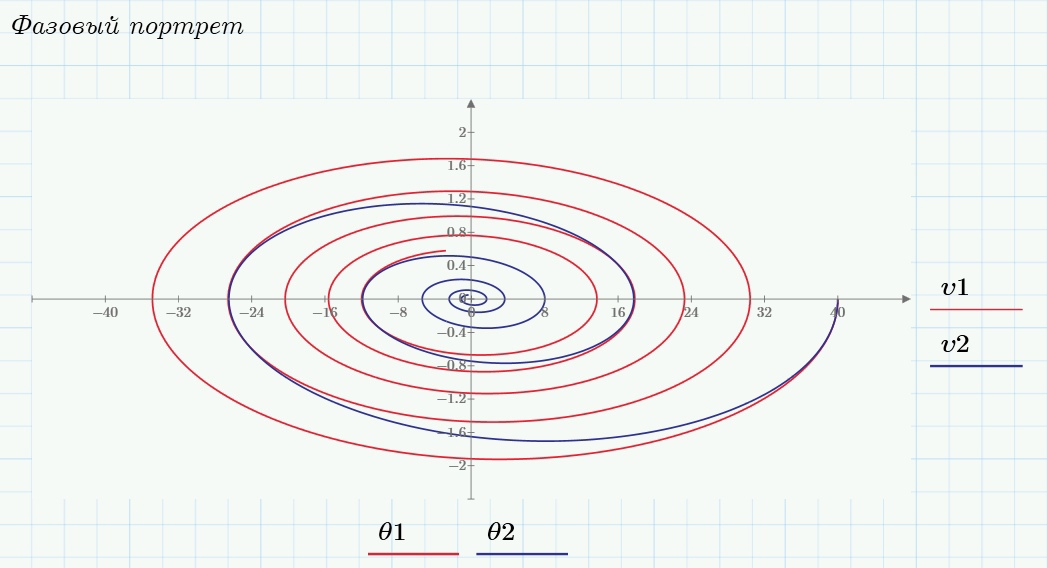
\includegraphics[width = \linewidth]{15.jpg}
			\caption[.] {Фазовый портрет при $\theta = 40^{\circ}$ $k = 0.25$ и $k=0.75$}
		\end{figure}
	\pagebreak
	\subsection{Вынужденные колебания}
		\begin{figure}[H]
			\centering
			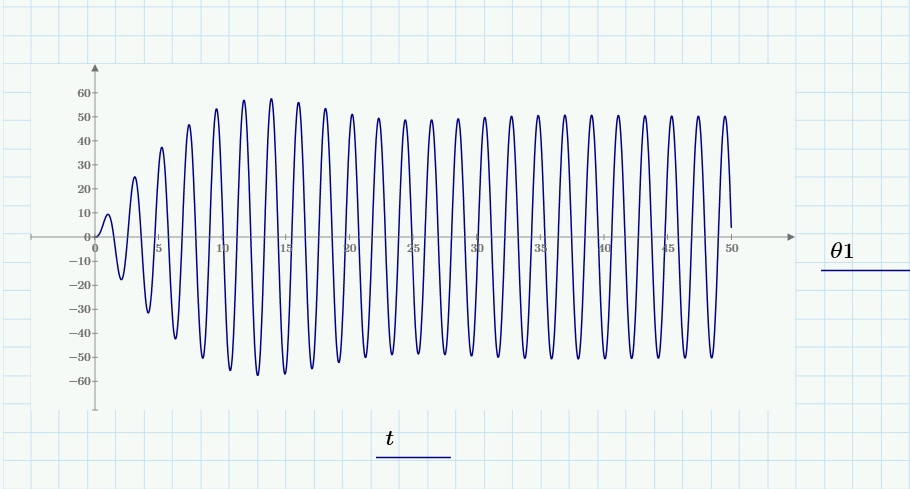
\includegraphics[width = \linewidth]{17.jpg}
			\caption[.] {График вынужденных колебаний}
		\end{figure}
		\subsection{Резонанс}
		\begin{figure}[H]
			\centering
			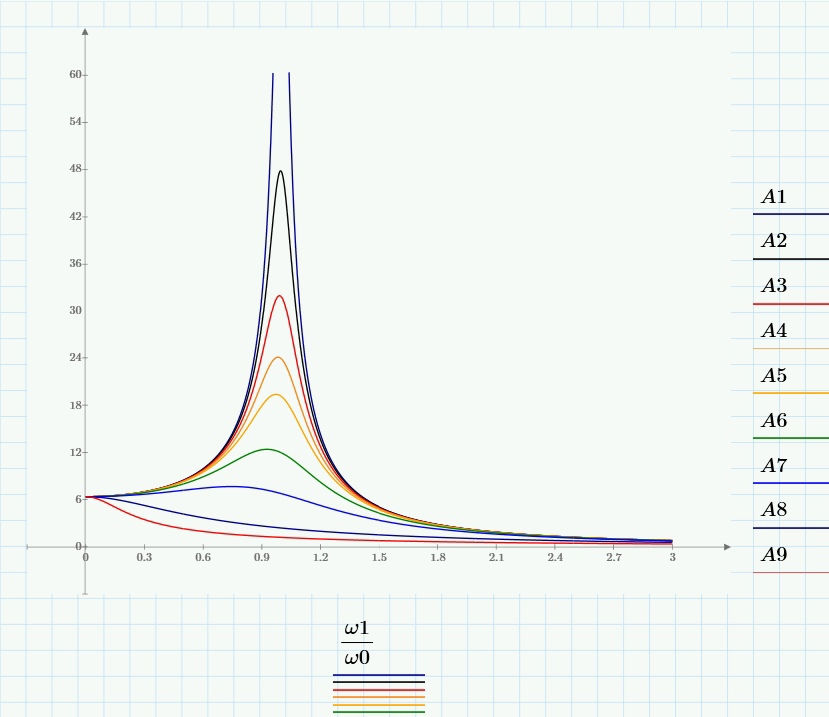
\includegraphics[width = \linewidth]{18.jpg}
		\end{figure}
		При $\omega_0 = \omega$ возникает резонанс.
		
	\section{Вывод}
		Таким образом, были составлены математические модели линейных и нелинейных незатухающих, затухающих и вынужденных колебаний. 
		
\end{document}	